
\chapter{Introduction}

\section{Intracellular transport}
%\blindtext \index{example1}
 You can reference a text using \parencite{fu2013}, or multiple citations using \parencite{klopfenstein2004, kumar2019, mahajan2019}.
 
 
\begin{figure}[H]
	\centering
	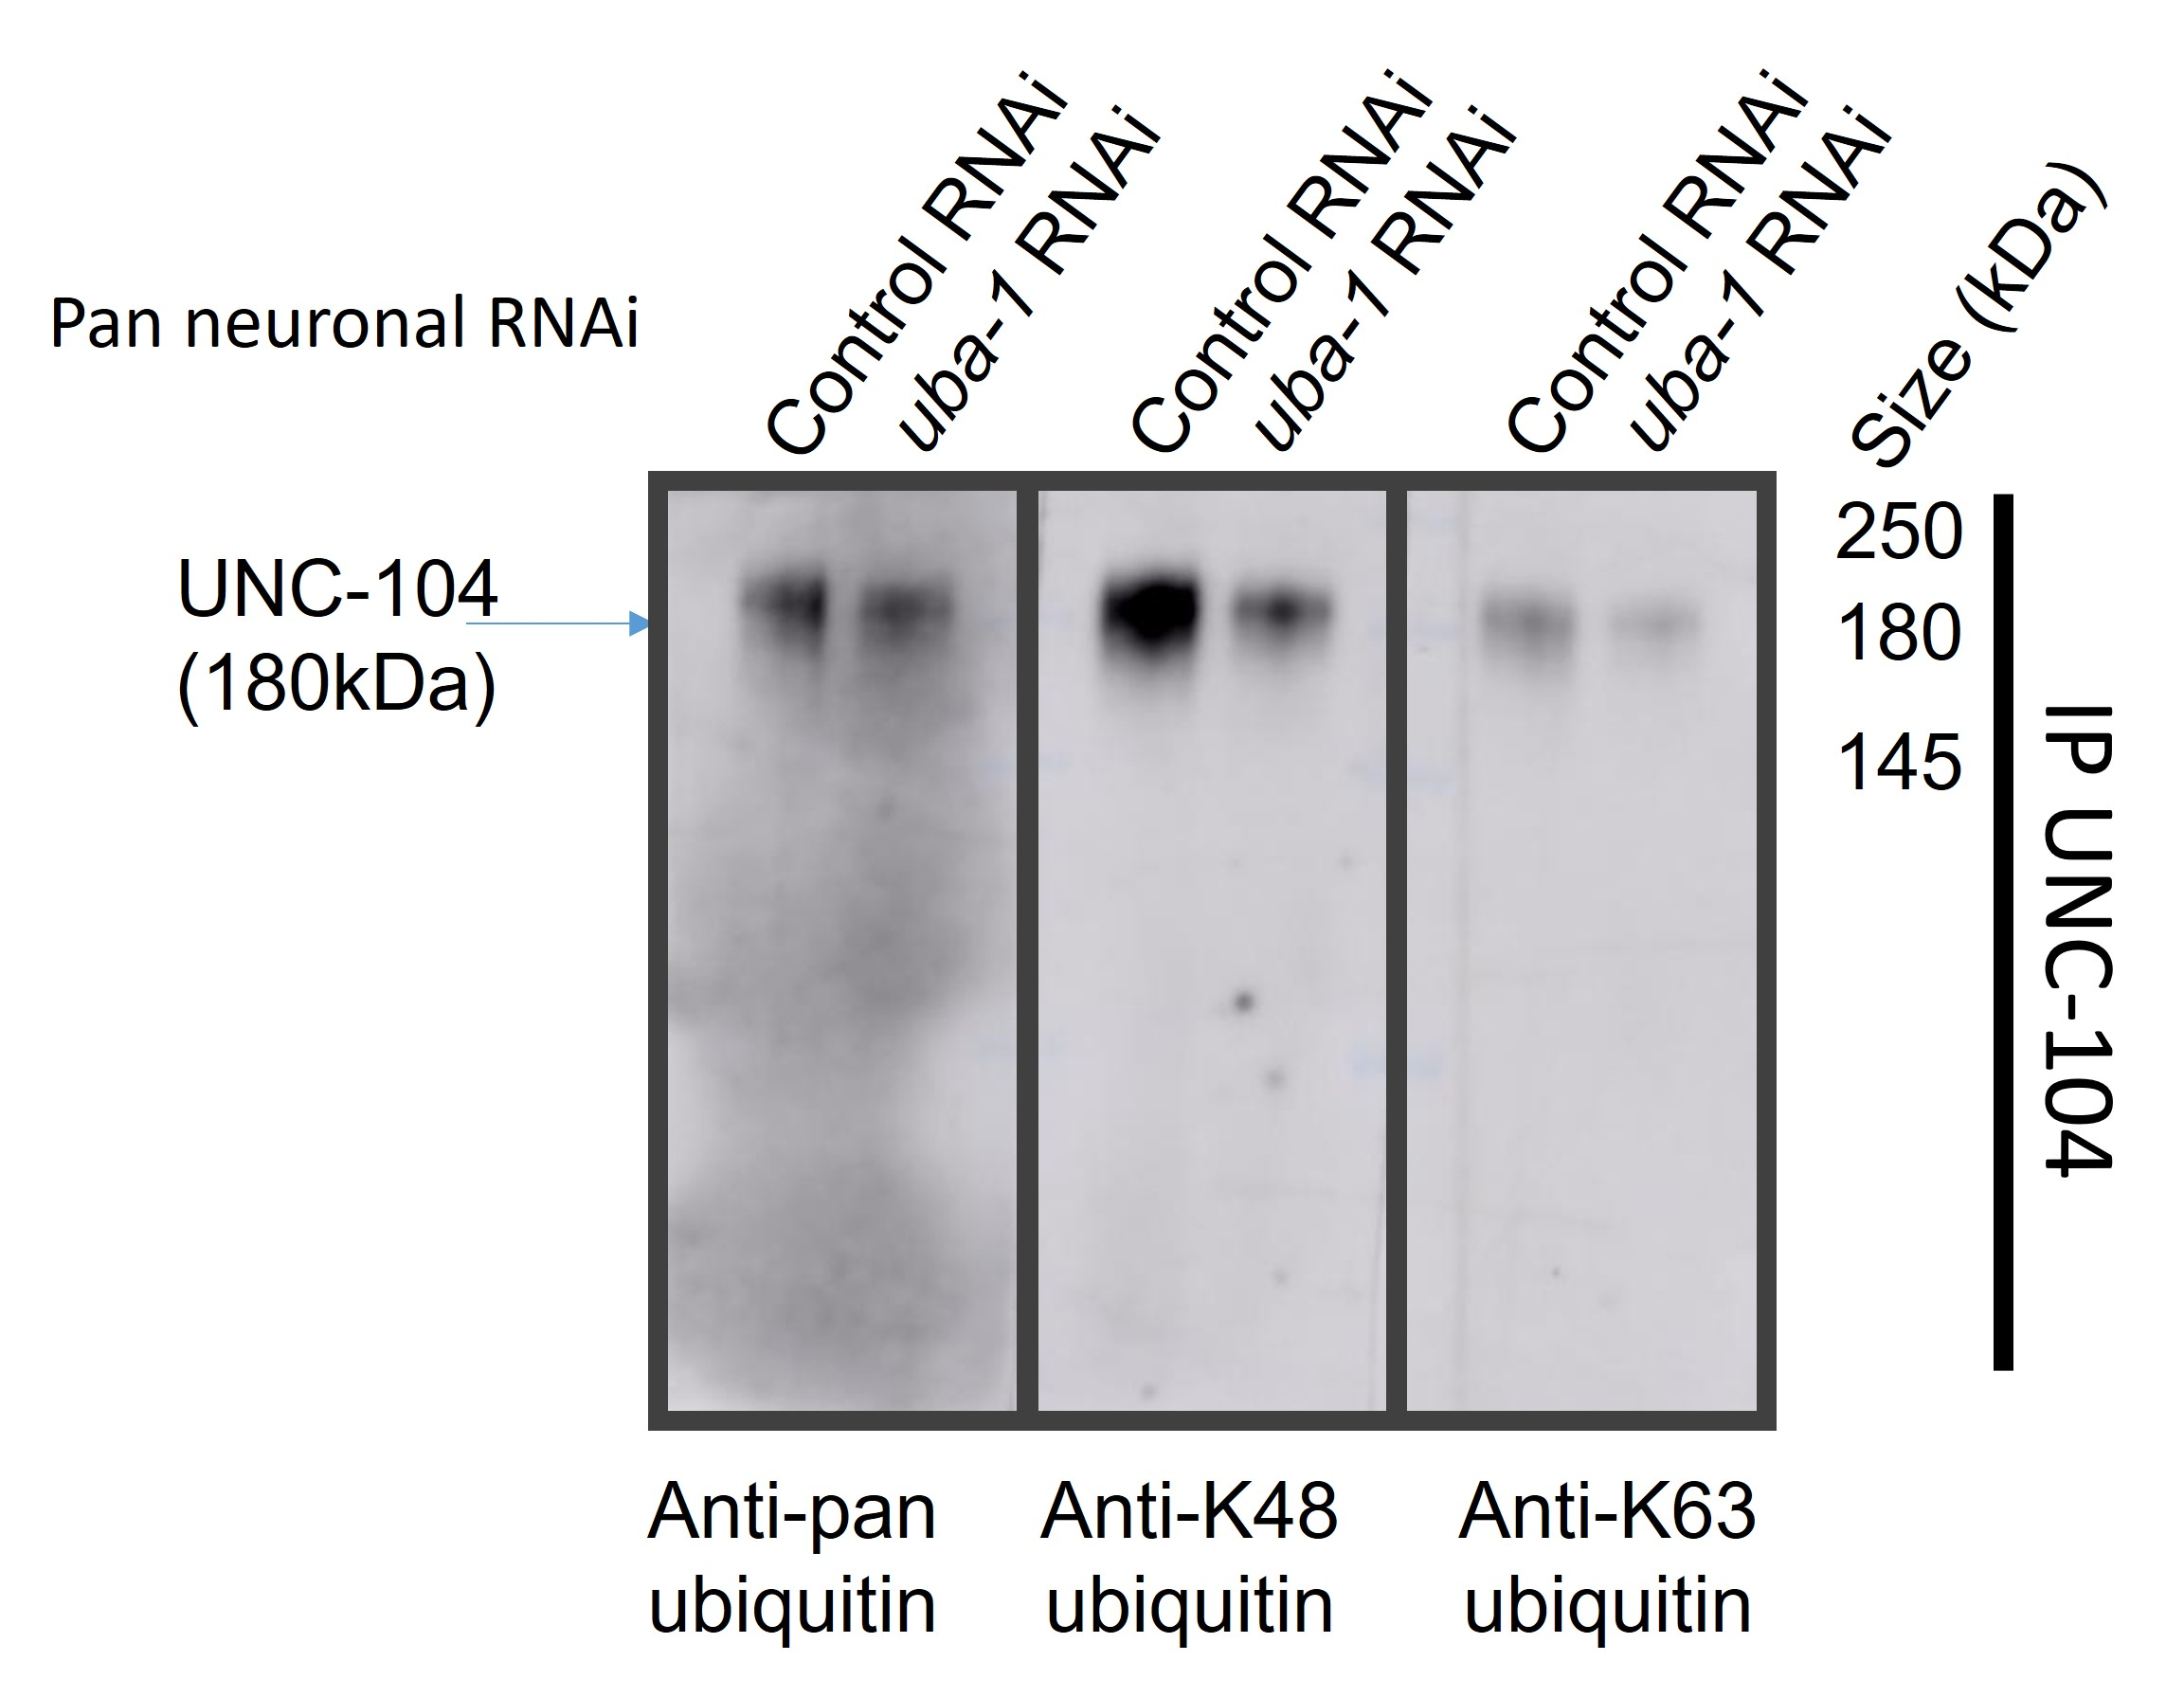
\includegraphics[width=\textwidth]{figs/example}
	
	\caption[Mechanism that contribute to compartment specific transport.]{\textbf{Mechanism that contribute to compartment specific transport.}} \raggedright \small Schematic representation of different examples of mechanisms that may regulate location specific transport of various kinesin members in a neuron. The mechanisms include 1) differentially modified MT indicated as red and blue lines that drive selective transport, 2) the axon initial segment (AIS) marked in the proximal axon that may act as a selective barrier, and 3) enrichment of kinesins at particular locations such as within the cilia.
 	\label{fig:Ch1f1}
\end{figure}

You can use an acronym by the gls command \gls{NRX-1}. Only after referencing an acronym will it show in the acronym list.

You can also use math symbols such as $\sim$10 $\mu$m.

You can reference a figure using [Fig.~\ref{fig:Ch1f1}]. A similar code can be used for an element you label using the label command.

You can also leave a personal comment using \marginpar{Neuronal migration?}.

You can leave bullet points with:-
\begin{enumerate}
	\item First point 
	
	\item Second point

	\item Third point

\end{enumerate}


Equations can be added in Latex format
\begin{equation}
	\label{dyn2}
	\partial_t \frac{C(x,t)}{C_{0}} + v \partial_x \frac{C(x,t)}{C_{0}}  - D \partial_x^2 \frac{C(x,t)}{C_{0}}  = 0, \nonumber
\end{equation}

These equations can be referenced [Fig.~\ref{dyn2}]. 

\textcolor{red}{You can highlight text using this command}

You can also add equations inline using  $\frac{C(x,t)}{C_{0}}$. i

\section{Table Example}
\blindtext \index{example2}

You can add a table using the following format.
\begin{table}[ht]
	\centering
	\caption{Closest orthologue of selected E3s} \label{tab:E3sselected}
	\begin{tabular}{|c|c|c|}
		\hline 
		Phenotype	& \textit{C. elegans} gene& Closest mammalian orthologue \\[0.5ex] 
		\hline\hline 
		Distal end UNC-104 accumulation	& \textit{fbxa-81} & FBXL13 \\ 
		\hline 
		Distal end UNC-104 accumulation	& \textit{fbxb-65} & FBW1A\\ 
		\hline 
		Distal end UNC-104 accumulation	& C10E2.2& FBXO30\\ 
		\hline 
		Synapse UNC-104 accumulation & \textit{fbxb-35}& NIL\\ 
		\hline 
		Synapse UNC-104 accumulation & \textit{fbxa-103}& NIL\\ 
		\hline 
	\end{tabular}
	
\end{table}
\blindtext 


A specially formatted table that have different column widths and can continue for multiple pages
\newcolumntype{L}{>{\RaggedRight\hangafter=1\hangindent=1.5em}X}
\begin{table}[H]\centering
	\caption{Strain list used in this chapter}\label{tab:Strainlist2}
	\scriptsize
	\begin{tabularx}{1\textwidth}{@{} l l L l @{}}\toprule
		S. No. &Strain name &Genotype &Reference \\\midrule
		1 &NM2689 &\textit{jsIs821 [mec-7p::gfp::rab-3]} &\cite{bounoutas2009} \\
		2 &NM3764 &\textit{jsIs1111 (mec-4p::unc-104::gfp)} &\cite{kumar2010} \\
		3 &TU3568 &\textit{sid-1(pk3321) him-5(e1490)} V; \textit{lin-15B(n744)} X; \textit{uIs71 [(pCFJ90) myo-2p::mCherry + mec-18p::sid-1]} &\cite{calixto2010} \\
		4 &RV110 &\textit{uba-1(it129ts)} &\cite{kulkarni2008} \\
		5 &TT343 &\textit{tbIs147} [Integrated line of \textit{mec-4p::UNC-104::GFP} in e1265 background] &\cite{kumar2010} \\
		6 &TT2980 &\textit{tbEx409 [mec-4p::mScarlet]} &This study \\
		7 &TT2228 &\textit{tbEx275} [\textit{mec-4p::UNC-104::GFP}(TTpl506)(5ng/ul) + \textit{ttx-3p::RFP}(TTpl541)(50ng/ul)+ pBluescript SK-(TTpl542)(200ng/ul)] &This study \\
		8 &TT2319 &\textit{tbEx276} [\textit{mec-4p::UNC-104 deltaPH::GFP}(TTpl567)(5ng/ul) + \textit{ttx-3p::RFP}(TTpl541)(50ng/ul)+ pBluescript SK-(TTpl542)(200ng/ul)] &This study \\
		9 &TT2353 &\textit{tbEx281} [\textit{mec-4p::UNC-104(M1540I)::GFP}(TTpl570)(5ng/ul) + \textit{ttx-3p::RFP}(TTpl541)(50ng/ul)+ pBluescript SK-(TTpl542)(200ng/ul)] &This study \\
		10 &TT2355 &\textit{tbEx279} [\textit{mec-4p::UNC-104(D1497N)::GFP}(TTpl569)(25ng/ul) + \textit{ttx-3p::RFP}(TTpl541)(50ng/ul)+ pBluescript SK-(TTpl542)(100ng/ul)] &This study \\
		11 &TT2399 &\textit{tbEx287} [\textit{mec-4p::UNC-104(D1497N M1540I)::GFP}(TTpl578)(3ng/ul) + \textit{ttx-3p::RFP}(TTpl541)(50ng/ul)+ pBluescript SK-(TTpl542)(200ng/ul)] &This study \\
		12 &TT2398 &\textit{tbEx289} [\textit{mec-4p::GFP}(TTpl581)(1ng/ul) + \textit{ttx-3p::RFP}(TTpl541)(50ng/ul)+ pBluescript SK-(TTpl542)(200ng/ul)] &This study \\
		13 &TU3401 &\textit{sid-1(pk3321) uIs69 [(pCFJ90) myo-2p::mCherry + unc-119p::sid-1]} V &\cite{calixto2010} \\
		\bottomrule
	\end{tabularx}
\end{table}


% After each chapter you can add biblography.
% If you want only one Biblography, remove following helper file and put content of it in main.tex
%\clearpage
%% This is helper file which you can use in every chapter if you want to have separate biblography for each chapter

% If you want only single biblography for all thesis, just copy paste following content at the end of main.tex

%	\bibliographystyle{unsrt}
%	\bibliography{Thesis}

	\printbibliography
	